\lecture[LoRaWAN]{LoRa and LoRaWAN}{LoRaWAN}

\nopartpage
\part{LoRaWan Topology, Technology and Properties}
\withpartpage

\begin{frame}{LoRaWAN Topology}
  \alert{LoRaWan} is an abbreviation for \alert{Long Range Wide Area Network}
  \begin{itemize}
    \item Typically \alert{\SI{10}{\kilo\meter}} using a \alert{\SI{0.25}{\milli\watt}} transceiver.
    \item \href{https://www.thethingsnetwork.org/article/new-lora-world-record-1336-km-830-mi\#:~:text=The\%20long\%20term\%20LoRaWAN\%C2\%AE,at\%201336\%20km\%20\%2F\%20830\%20miles.}{World record}: \alert{\SI{1336}{\kilo\meter}}.
  \end{itemize}
  \begin{center}
    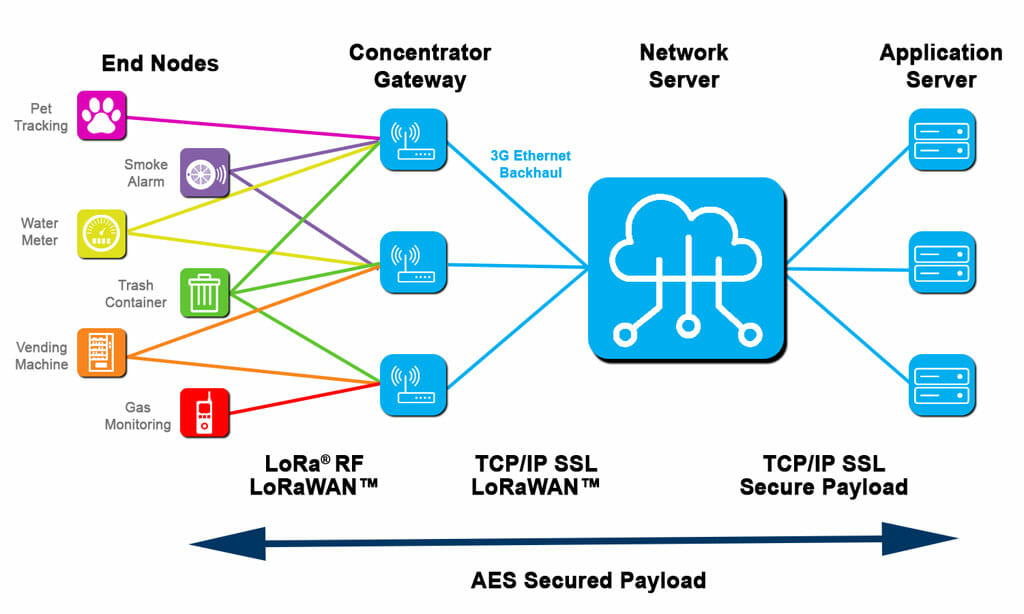
\includegraphics[width=0.7\textwidth]{material/lorawan-topography.jpg}
  \end{center}
\end{frame}
